\section{EXPERIMENTAL SETTING AND RESULTS}
\label{sec:mot}
\begin{figure}
	\centering
	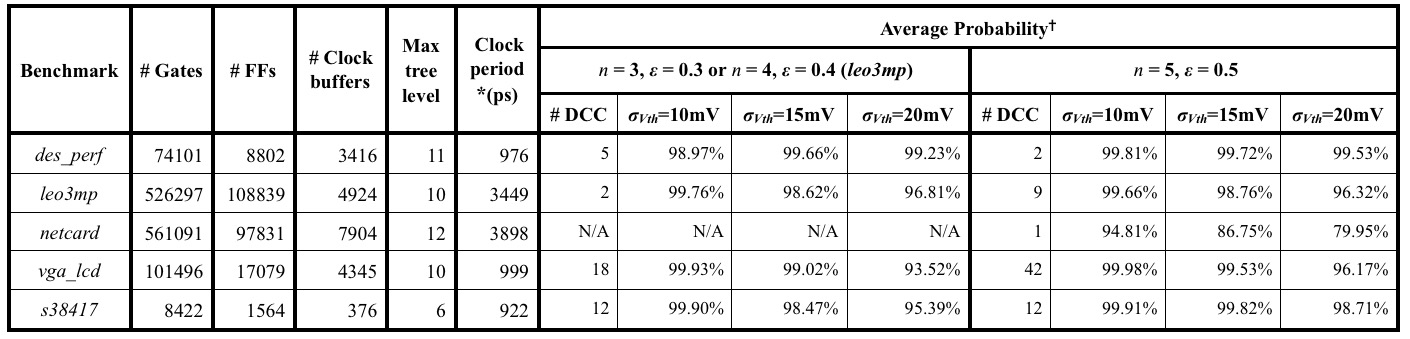
\includegraphics[width=1\columnwidth]{./experiment/benchmarkinfo.png}
	\caption{Circuit information and estimated lifetime without Trojan insertion}
	\label{fig:benchmark}
\end{figure}

%%---------TEST--------------
\begin{figure*}[!ht]
    \centering
    \subfigure[\textit{s38417} is attacked with $n$ = 3 yr and $\varepsilon = 0.3$ yr]{
    	\label{fig:sub:s38417_3y}
        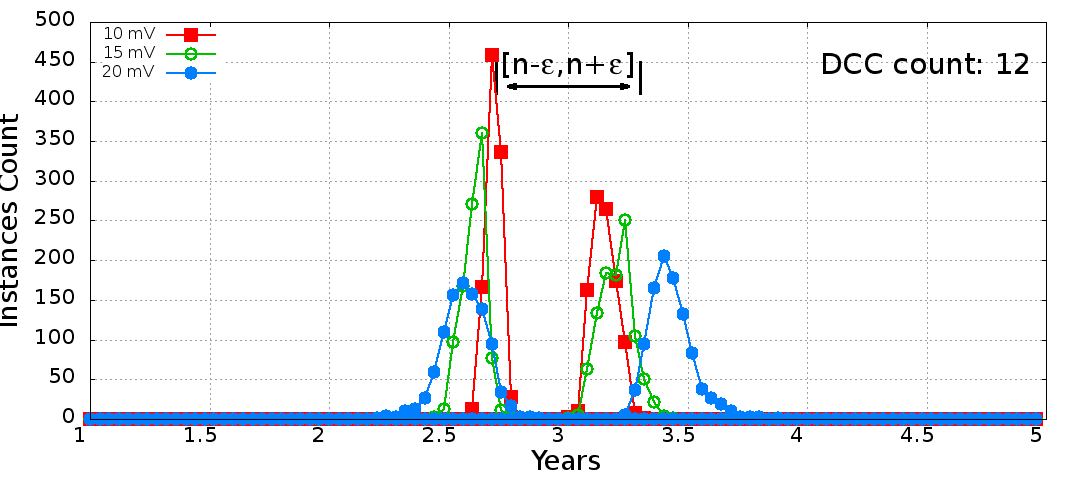
\includegraphics[width=0.8\columnwidth]{./experiment/s384173y.png}
    }
    \hspace{0.1cm}
    \subfigure[\textit{s38417} is attacked with $n$ = 5 yr and $\varepsilon = 0.5$ yr]{
    	\label{fig:sub:s38417_5y}
        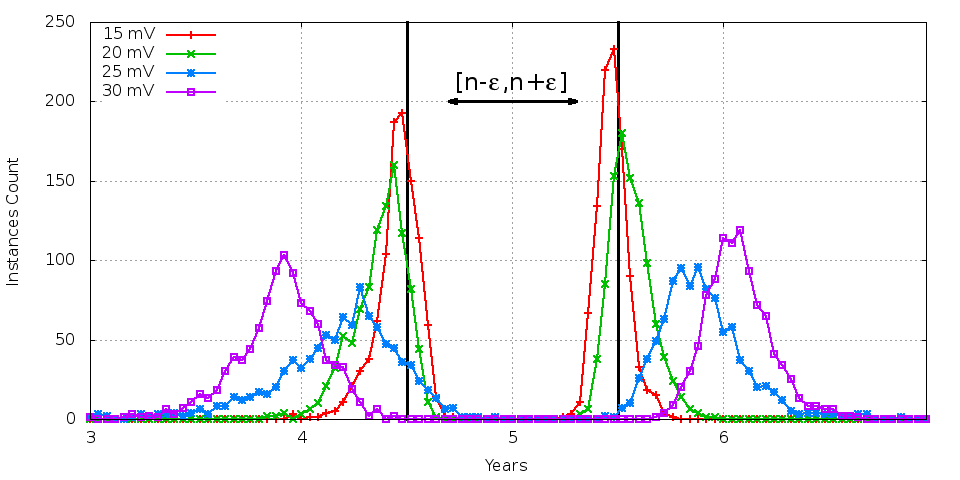
\includegraphics[width=0.8\columnwidth]{./experiment/s384175y.png}
    }
    \hspace{0.1cm}
    \subfigure[\textit{des\_perf} is attacked with $n$ = 3 yr and $\varepsilon = 0.3$ yr]{
    	\label{fig:sub:des_3y}
        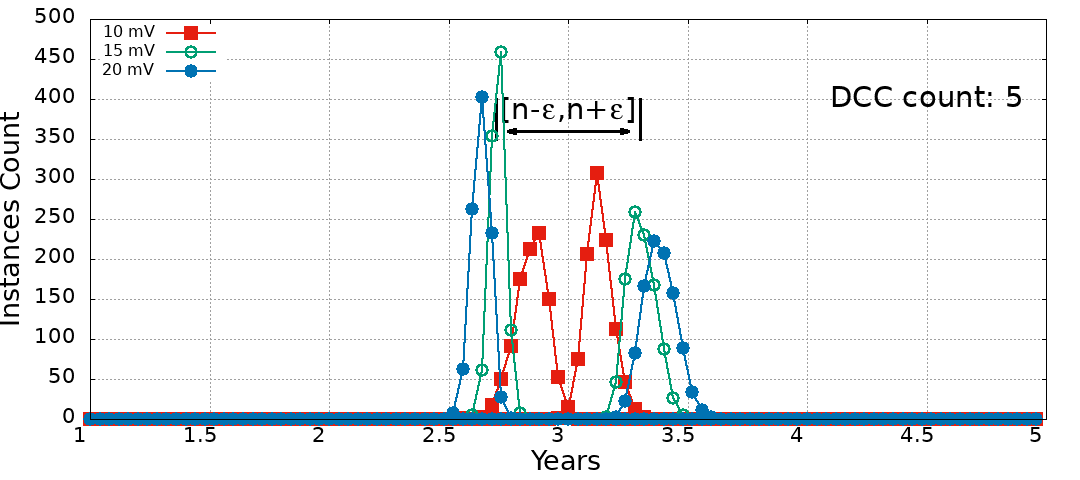
\includegraphics[width=0.8\columnwidth]{./experiment/des3y.png}
    }
    \subfigure[\textit{des\_perf} is attacked with $n$ = 5 yr and $\varepsilon = 0.5$ yr]{
    	\label{fig:sub:des_5y}
        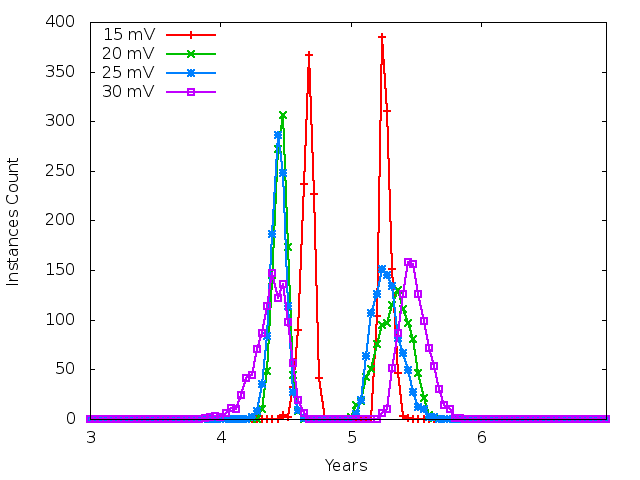
\includegraphics[width=0.8\columnwidth]{./experiment/des5y.png}
    }
    \subfigure[\textit{leo3mp} is attacked with $n$ = 4 yr and $\varepsilon = 0.4$ yr]{
    	\label{fig:sub:3mp_3y}
        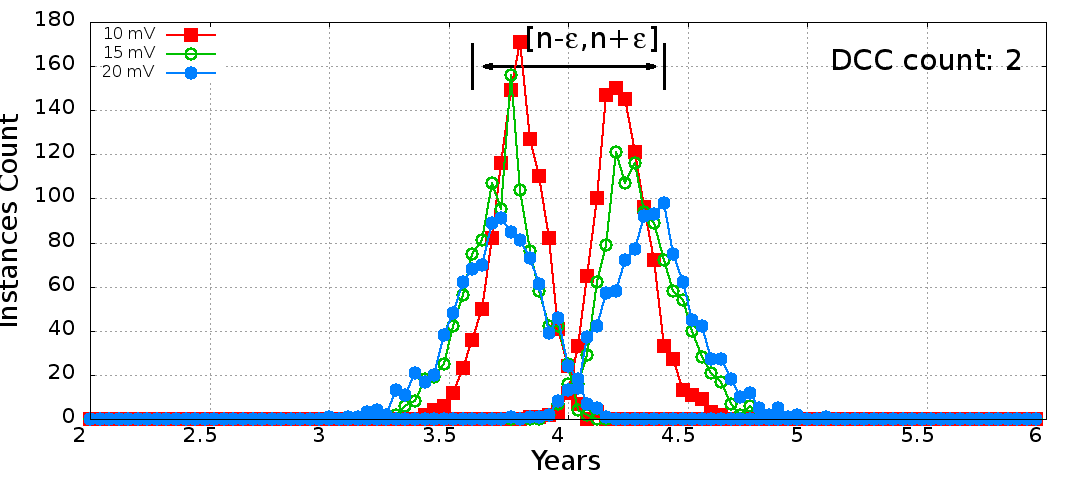
\includegraphics[width=0.8\columnwidth]{./experiment/3mp4y.png}
    }
    \hspace{0.1cm}
    \subfigure[\textit{leo3mp} is attacked with $n$ = 5 yrs and $\varepsilon = 0.5$ yr]{
    	\label{fig:sub:3mp_5y}
        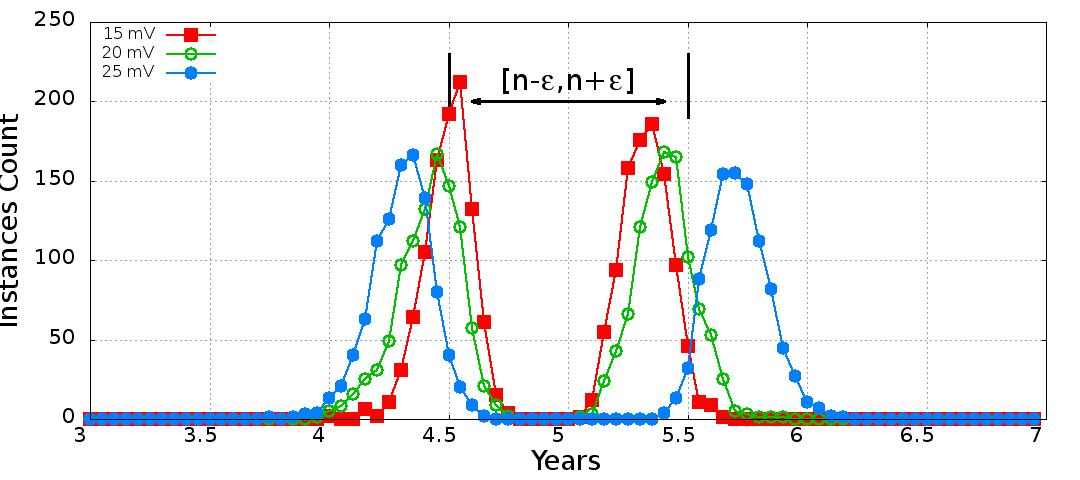
\includegraphics[width=0.8\columnwidth]{./experiment/3mp5y.png}
    }
    \caption{Lifetime distributions of Monte-Carlo Instances of \textit{s38417}, \textit{des\_perf}, and \textit{leo3mp}}
    \label{fig:exp}
\end{figure*}


In this section, we explain the experimental setting and demonstrate the experimental result of our proposed Trojan attack. The benchmarks are picked out from IWLS'05 and ISCAS'89 for the experiments. The utilized technology is TSMC 65nm GP standard cell series. The used SAT solver is MiniSAT 2.2. %The section is organized as follows: Section~\ref{sec:exp:tc} introduces the experimental setting for clock period. Section~\ref{sec:exp:exp} demonstrates the lifetime distributions of Monte-Carlo instances of attacked designs, Eventually, Section~\ref{sec:exp:det} discuss the detectability of the proposed Trojan attack.  

\subsection{Clock Period Setting}
\label{sec:exp:tc}
As shown in Figure \ref{fig:benchmark}, column 7 shows the lifetime intervals of original (i.e., Trojan-free) designs with the corresponding clock periods (in column 6) which make the designs fail at the specified time (in our experiment, 7 years) under aging. The resulting clock period is both used in Trojan-free and Trojan-included (attacked) designs. In Figure~\ref{fig:benchmark}, lifetime lower bounds are exactly 7 years because the clock period (shown in column 4) of each design is specifically set such that the most critical path will fail at $7^{th}$ year under the severe aging condition. The upper bound of each design varies with the workload variations, from time to time.

\subsection{Monte-Carlo Instantiation of the Attacked Designs}
\label{sec:ins:mc_ins}
Given an attacked design, each Monte-Carlo instance of the design is generated by imposing extra V\textsubscript{th} offset (i.e., $\Delta V\textsubscript{th}$ ) on each transistor. The offsets follow a normal distribution with the standard deviation of a given value (usually 10mV - 25mV~\cite{han2011statistical}\cite{schlunder2017influence}). Each instance (i.e., Monte-Carlo seed) can be viewed as a die. In our experiment, each attacked design is instantiated for 1000 times with a specified standard deviation of V\textsubscript{th}. 

\subsection{Lifetime Estimation Considering the Effect of PVs on Aging Rates of Transistors}
\label{sec:ins:lt}
Whenever an instance is generated, we estimate the lifetime interval of the instances. Note that, because threshold voltages of transistors are not the same due to PVs, their aging rates differ with each others. As a consequence, we cannot use the deterministic Equation (\ref{eq:worst}) to derive the severe aging rates of candidate paths. Instead, we derive the aging rate of individual transistor based on the mathematical model in Section~\ref{sec:frame} regarding the correlation between PVs and BTI.

\subsection{Lifetime Distribution of Monte-Carlo Instances}
\label{sec:exp:exp}
Figure~\ref{fig:exp} shows the lifetime distributions of instances of the attacked three designs (\textit{s38417}, \textit{des\_perf} and \textit{leo3mp}). The designs are attacked to fail at $3^{rd}$, $4^{th}$ or $5^{th}$ year. Note that, there exists no SAT solution while \textit{leo3mp} is attacked to fail at $3^{rd}$ year, whereas there exists SAT solution while it is attacked to fail at $4^{th}$ year. In each subfigure, there exist three distributions, each of distributions corresponds to one standard deviation of V\textsubscript{th} while generating Monte-Carlo instances. In our experiments, the deviations are set to 15mV, 20mV, and 25mV, respectively. As we can observe in each distribution, there exist two peaks, which indicate lower/upper bounds of lifetime intervals of instances. Note that, there exist two differences between Figure~\ref{fig:benchmark} and Figure~\ref{fig:exp}. First, the designs in Figure~\ref{fig:benchmark} are Trojan-free ones, instead of Trojan-included ones in Figure~\ref{fig:exp}. Second, because the lifetime intervals of the Trojan-free designs are not subject to the PVs, the original lifetime intervals ($7^{th}$ column in Figure~\ref{fig:benchmark}) do not consider the effect of PVs.

As shown in Figure~\ref{fig:exp} apparently, as the standard deviation becomes larger, the interval between the left and right peaks becomes wider, indicating the larger standard deviation leads to fewer accurate attacks. Therefore, the lifetime accuracy of the proposed Trojan is impacted by the diversity of threshold voltages of transistors. Even though the peaks of two bounds deviate from the desired lifetime interval $[n - \varepsilon, n + \varepsilon]$, as mentioned in Section~\ref{sec:frame}, it does not mean that the attacked designs must not fail in that interval. The exact fail time point depends on the workload. Since the lifetime interval of each instance is overlapped with the desired lifetime interval $[n - \varepsilon, n + \varepsilon]$, the proposed Trojan is still likely to control the design lifetime in that interval.

\subsection{Detectability}
\label{sec:exp:det}
A side-channel analysis is a countermeasure often taken for detecting the existence of hardware Trojan. Nevertheless, the used DCC count is marginal compared with the total gate count. On average, DCC count is less than 0.2\% of total gate count. That is, the area overhead is insignificant. In addition, the power overhead due to DCCs can be regarded as the power variations caused by PVs. As a result, the proposed Trojan is difficult to detect by the conventional side-channel analysis. 

Some Trojan defenders can insert on-chip monitors in the clock network to inspect the variation of clock duty cycle. However, the method need extra I/O pins/ports, which is impractical because the pin counts of ICs are limited and the area overhead.


\section{CONCLUSION}
We proposed a framework of hardware Trojan insertion to control the circuit lifetime with the consideration of aging behavior, correlation between pairs of critical paths and process variations. The influence of Trojan heavily reduce the lifetime of circuit instances. Even though the accuracy is impacted by PVs, the lifetime of instances is still likely to fail within the desired lifetime interval $[n - \varepsilon, n + \varepsilon]$. More important, the area overhead of inserted DCCs is less than an average of 0.2\% of total gate count, which implies the proposed Trojan is very difficult to detect and succeed in decreasing the lifetime of attacked designs.
